\documentclass[paper=a4, fontsize=11pt]{scrartcl} % A4 paper and 11pt font size
\usepackage[T1]{fontenc}  % proper encoding for output file
\usepackage[utf8]{inputenc}  % except UTF-8 character in source
\usepackage[english]{babel}  % set document language
\usepackage{amsmath,amsfonts,amsthm}  % math type setting
\usepackage{mhchem}  % chemical expressions
\usepackage{graphicx}  % inclue graphics
\usepackage{url}
\usepackage{caption}
\usepackage{subcaption}
\setlength\parindent{0pt} % Removes all indentation from paragraphs


\title{Exercise 4: Atmospheric Brightness Temperature Spectra}
\author{Sample Solution}
\date{Effective: 26.01.2017}

%%%%%%%%%%%%%%%%%%%%%%%%%%%%%%%%%%%%%%%%%%%%%%%%%%%%%%%%%%%%%%%%%%%%%%%%%%%%%%%
\begin{document}

\maketitle

1. Use the ARTS control file \texttt{rtcalc.arts} and Matlab plotting script
\texttt{plot\_bt.m} to calculate and display the spectrum of atmospheric zenith
opacity in the microwave spectral range for a midlatitude-summer atmosphere.
There are four spectral lines in the plot. 

\textbf{Questions}
\begin{itemize}
  \item To which species do these lines belong? (You can find this out by
      playing with the absorption species selection in the ARTS control file.)
  \item We speak of window regions where the zenith opacity is below 1. Where
      are they?
\end{itemize}

\begin{figure}[ht]
  \centering
  \begin{subfigure}[t]{0.45\textwidth}
  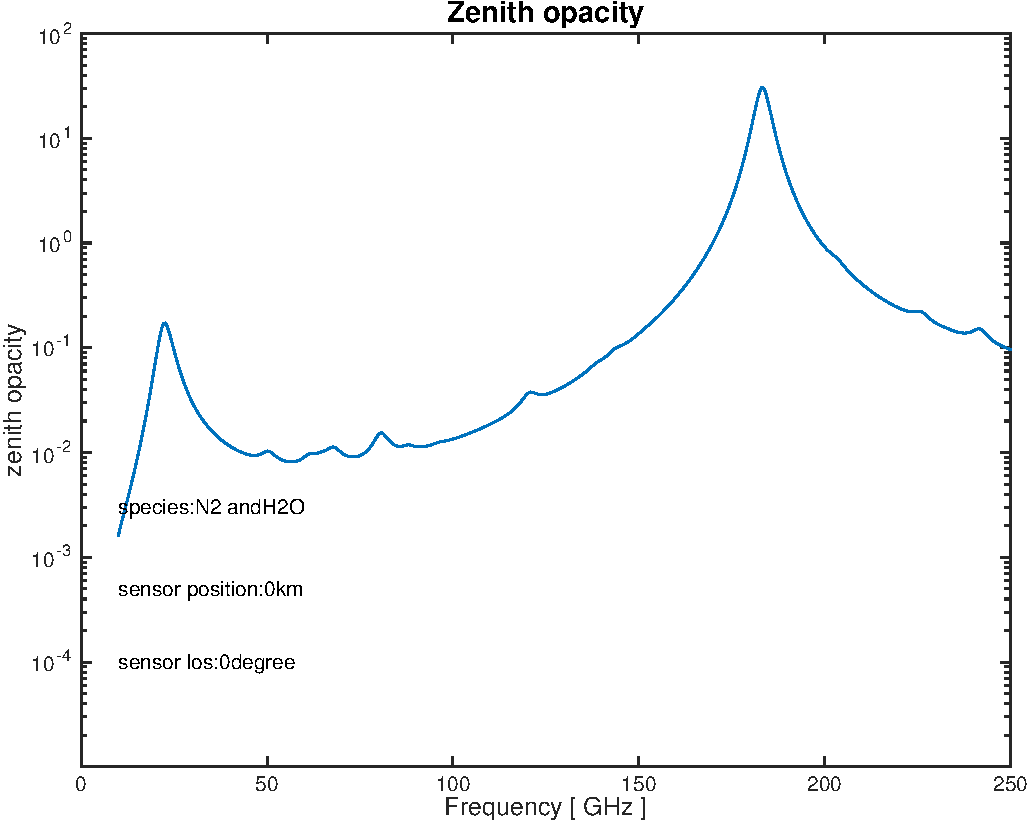
\includegraphics[width=\textwidth]{plots/opacity_N2+H2O_0km_0deg.pdf}
  \caption{\ce{H2O} and \ce{N2}}
  \end{subfigure}
  \begin{subfigure}[t]{0.45\textwidth}
  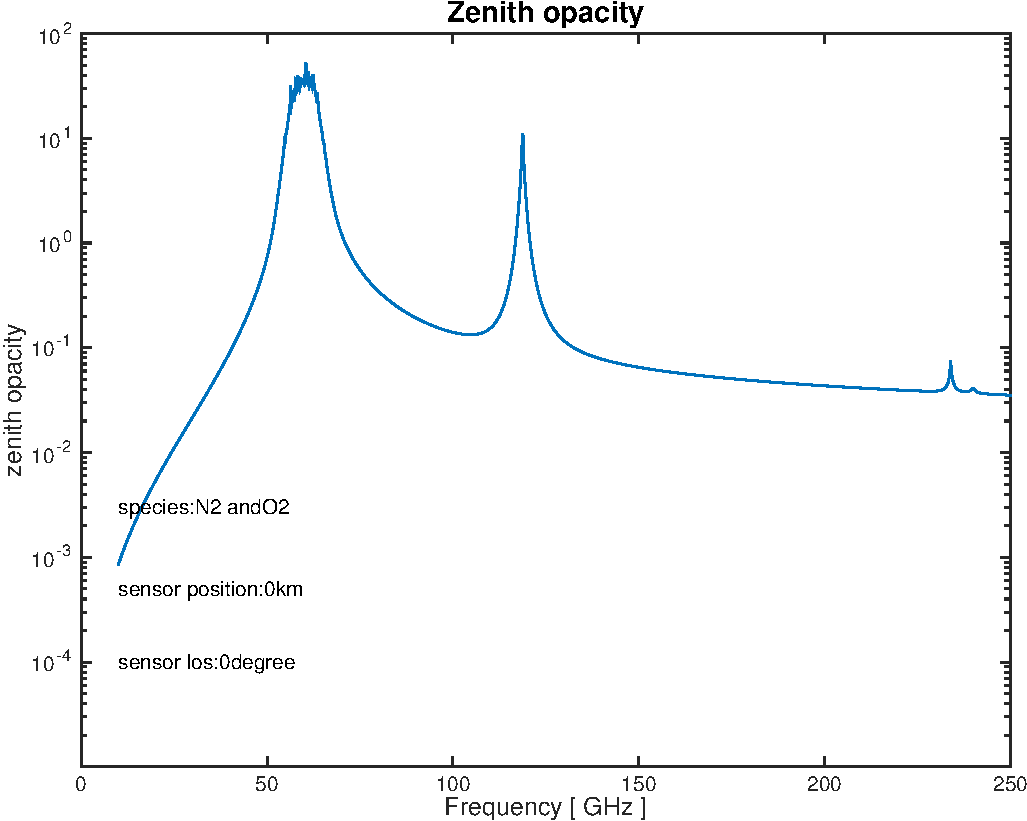
\includegraphics[width=\textwidth]{plots/opacity_N2+O2_0km_0deg.pdf}
  \caption{\ce{O2} and \ce{N2}}
  \end{subfigure}
  \caption{Zenith opacity separately for \ce{O2} and \ce{H2O} molecules.}
  \label{figure:abs_molucules}
\end{figure}

\begin{figure}[ht]
  \centering
  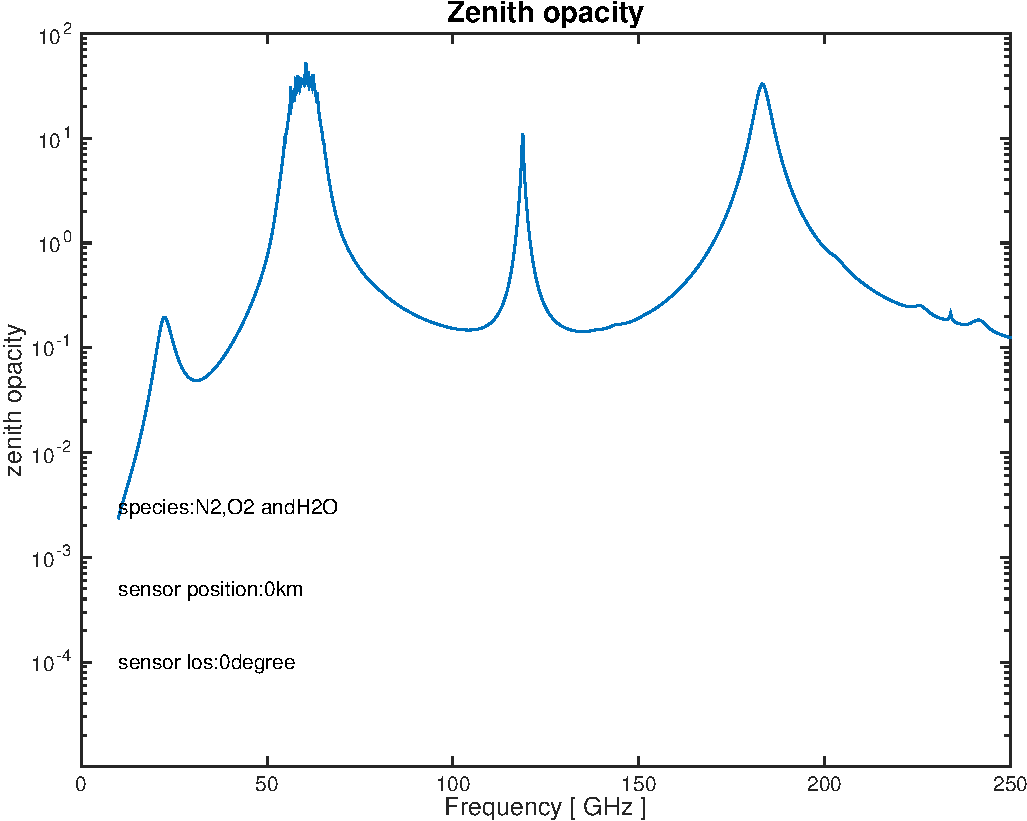
\includegraphics[width=\textwidth]{plots/opacity_N2+O2+H2O_0km_0deg.pdf}
  \caption{Zenith opacity.}
\end{figure}

\clearpage

2. Brightness temperature is a unit for intensity. It is the temperature that a
blackbody should have to give the same intensity as measured. Mathematically,
the transformation between intensity in SI units and intensity in brightness
temperature is done with the Planck formula. Calculate and display the
atmospheric brightness temperature spectrum for different hypothetical sensors:

\begin{itemize}
  \item A ground-based sensor looking in the zenith direction.
  \item A sensor on an airplane (z = 10\,km) looking in the zenith direction.
\end{itemize}

% figures abs cross sections
\begin{figure}[h]
  \centering
  \begin{subfigure}[h!]{0.45\textwidth}
    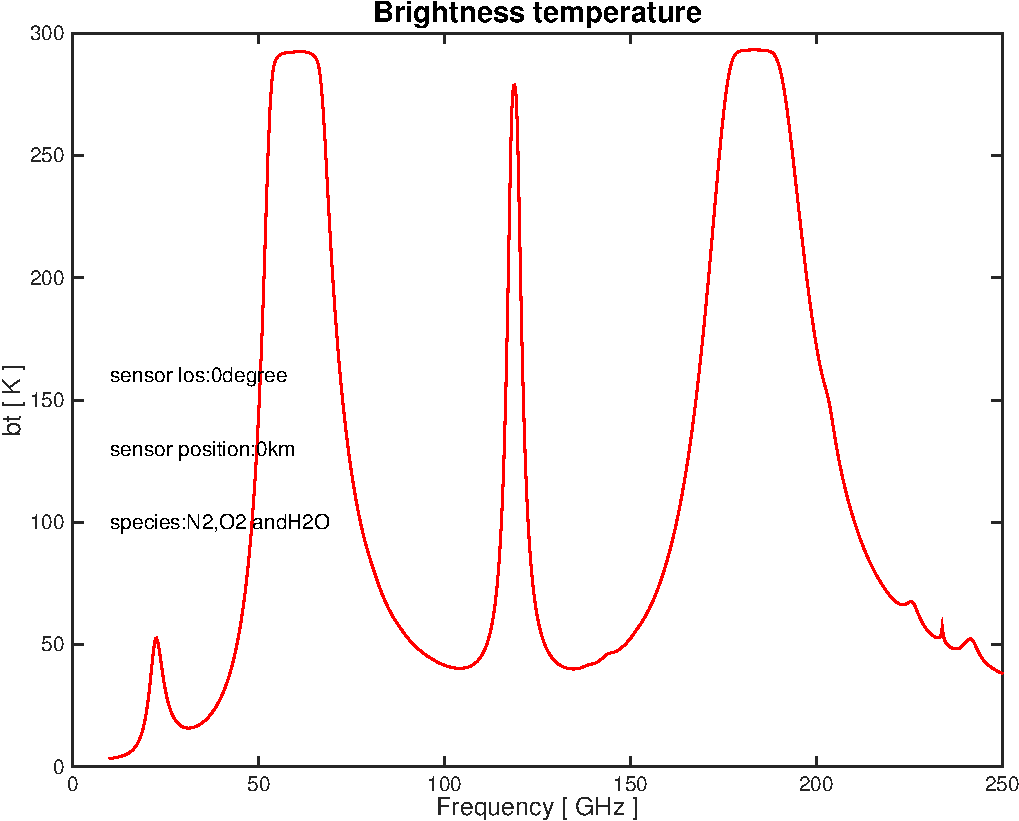
\includegraphics[width=\textwidth]{plots/bt_N2+O2+H2O_0km_0deg.pdf}
    \caption{Ground based.}
    \end{subfigure}
    \hfill    
    \begin{subfigure}[h!]{0.45\textwidth}
    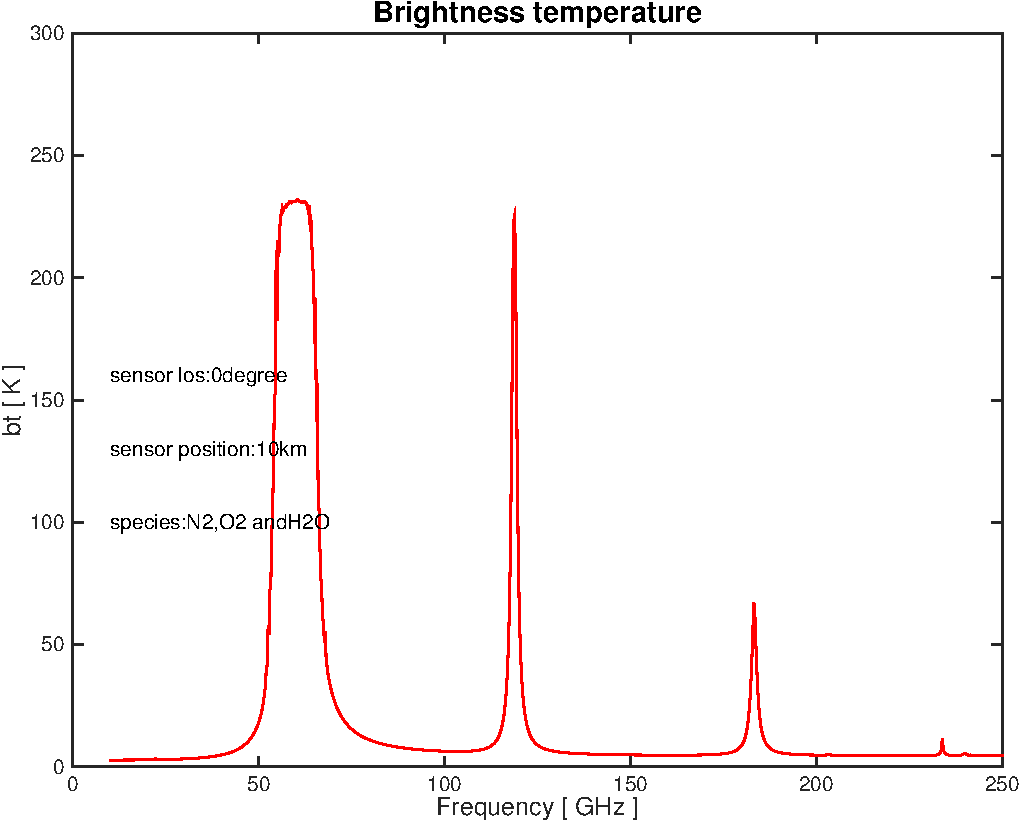
\includegraphics[width=\textwidth]{plots/bt_N2+O2+H2O_10km_0deg.pdf}
    \caption{10\,km height.}
    \end{subfigure}
  \caption{Brightness temperature for a sensor positioned at the ground and at
    10\,km height.}
  \label{figure:abs_pressure}
\end{figure}

\textbf{Questions}
\begin{itemize}
    \item In Plot (a), why do the lines near 60\,GHz and near 180\,GHz appear
        flat on top?
    \item In Plot (b), why is the line at 180\,GHz smaller than the line at
        120\,GHz, although its zenith opacity is higher?
    \item Describe the difference between plots (a) and (b). What happens to
        the lines, what happens to the background? Can you explain what you
        see?
\end{itemize}

\clearpage

3. Make the same calculation for a satellite sensor (z = 800\,km) looking nadir
(straight down).

\textbf{Questions}
\begin{itemize}
  \item Why is the line at 180\,GHz ``upside-down', but the one at 20\,GHz not?
  \item Explain the funny shape of the \ce{O2} line at 120\,GHz.
\end{itemize}

\begin{figure}[h]
\centering
 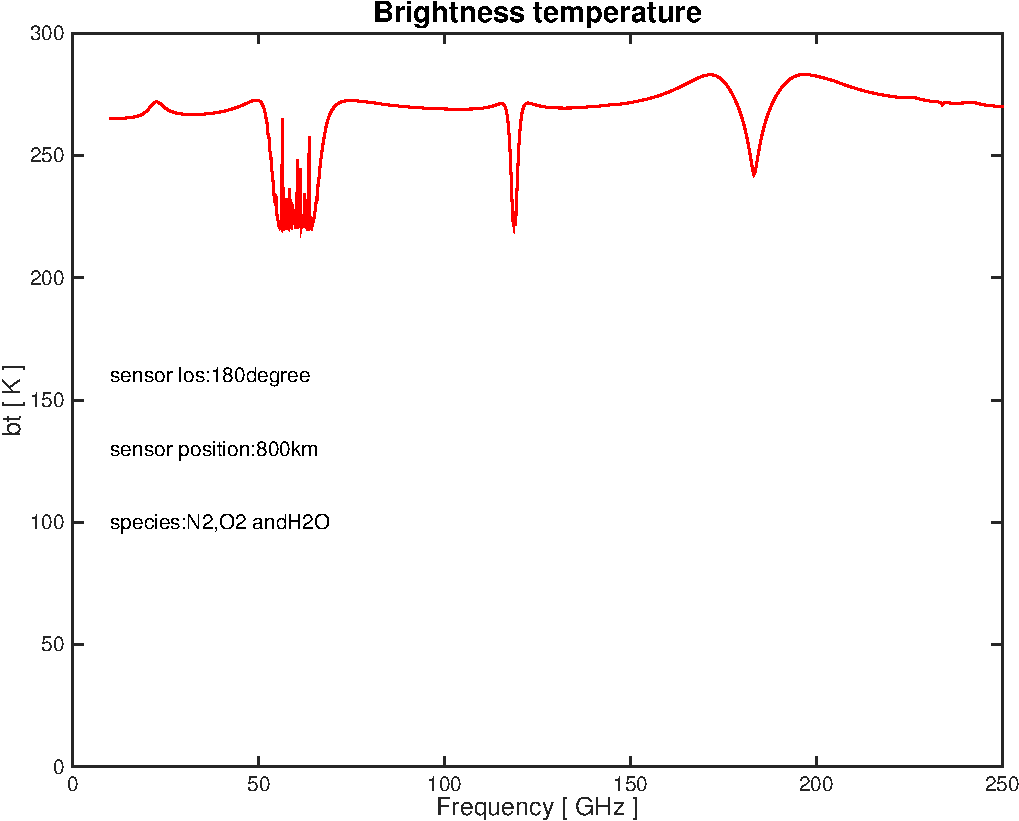
\includegraphics[width=\textwidth]{plots/bt_N2+O2+H2O_800km_180deg.pdf}
 \caption{Brightness temperature seen from a sensor looking down.}
\end{figure}
\end{document}
